
%\usepackage{wrapfig}

\resetcounters

\bibliographystyle{asp2010}

\markboth{Warner et al.}{Redefining the Data Pipeline Using GPUs}

\title{Redefining the Data Pipeline Using GPUs}
\author{C.~Warner,$^1$ S.~S.~Eikenberry,$^1$ A.~H.~Gonzalez,$^1$ and C.~Packham$^2$
\affil{$^1$University of Florida, Gainesville, FL}
\affil{$^2$University of Texas at San Antonio}}

\aindex{Warner, C.}
\aindex{Eikenberry, S. S.}
\aindex{Gonzalez, A. H.}
\aindex{Packham, C.}

\begin{abstract}
There are two major challenges facing the next generation of data processing pipelines: 1) handling an ever increasing volume of data as array sizes continue to increase and 2) the desire to process data in near real-time to maximize observing efficiency by providing rapid feedback on data quality.  Combining the power of modern graphics processing units (GPUs), relational database management systems (RDBMSs), and extensible markup language (XML) to re-imagine traditional data pipelines will allow us to meet these challenges.

Modern GPUs contain hundreds of processing cores, each of which can process hundreds of threads concurrently.  Technologies such as Nvidia's Compute Unified Device Architecture (CUDA) platform and the PyCUDA (\url{http://mathema.tician.de/software/pycuda}) module for python allow us to write parallel algorithms and easily link GPU-optimized code into existing data pipeline frameworks.  This approach has produced speed gains of over a factor of 100 compared to CPU implementations for individual algorithms and overall pipeline speed gains of a factor of 10-25 compared to traditionally built data pipelines for both imaging and spectroscopy (Warner et al., 2011).

However, there are still many bottlenecks inherent in the design of traditional data pipelines.  For instance, file input/output of intermediate steps is now a significant portion of the overall processing time.  In addition, most traditional pipelines are not designed to be able to process data on-the-fly in real time.

We present a model for a next-generation data pipeline that has the flexibility to process data in near real-time at the observatory as well as to automatically process huge archives of past data by using a simple XML configuration file.  XML is ideal for describing both the dataset and the processes that will be applied to the data.  Meta-data for the datasets would be stored using an RDBMS (such as mysql or PostgreSQL) which could be easily and rapidly queried and file I/O would be kept at a minimum.  We believe this redefined data pipeline will be able to process data at the telescope, concurrent with continuing observations, thus maximizing precious observing time and optimizing the observational process in general.  We also believe that using this design, it is possible to obtain a speed gain of a factor of 30-40 over traditional data pipelines when processing large archives of data.
\end{abstract}

\section{Introduction}
As we move into the era of Giant Segmented Mirror Telescopes (GSMTs)
and increasingly large surveys (e.g., panstarrs, dark energy survey, LSST), 
traditional data pipelines will be unable to handle the rapidly increasing
volume of data produced per night.  In addition, with telescope time becoming
more expensive than ever, there is a strong desire to maximize observing
efficiency by providing near real-time feedback on data quality via a
quick-look mechanism.  In order to meet both of these challenges, we must
not only speed up the data reduction process, but also fundamentally
redesign the traditional data pipeline model.

Modern Graphics Processing Units (GPUs) have been demonstrated to produce
speed gains of over a factor of 100 compared to CPU implementations for
individual algorithms that can benefit from massive parallelization (Warner
et al., 2011).  This is because modern GPUs have hundreds of multiprocessing
cores, each of which can process hundreds of threads concurrently.
GPU-optimized algorithms can be written using platforms such as Nvidia's
Compute Unified Device Architecture (CUDA).  These algorithms can be easily
linked into existing data pipeline frameworks by using either the PyCUDA
(\url{http://mathema.tician.de/software/pycuda}) module or Python's native
C-API, resulting in overall speed gains of a factor of 8-15 compared to
traditional CPU-based implementations of data pipelines (Table 1).

\begin{table}[!ht]
\caption{GPU-optimized speed gains}
\smallskip
\begin{center}
{\small
\begin{tabular}{lcccc}
\tableline
\noalign{\smallskip}
Data description & \# of Images & Time (s), CPU & Time (s), GPU & Speed-up\\
\noalign{\smallskip}
\tableline
\noalign{\smallskip}
Flamingos-I imaging (1-pass sky) & 60 & $754.8s$ & $62.4s$ & $12.1$\\
Flamingos-I imaging (2-pass sky) & 60 & $1035.5s$ & $121.6s$ & $8.5$\\
Flamingos-I MOS spectroscopy & 100 & $1601.1s$ & $202.3s$ & $7.9$\\
Flamingos-II imaging (2-pass sky) & 137 & $2031.5s$ & $247.9s$ & $8.2$\\
Flamingos-II longslit spectroscopy & 98 & $3181.8s$ & $242.4s$ & $13.1$\\ 
\noalign{\smallskip}
\tableline
\end{tabular}
}
\end{center}
\end{table}

However, implementation of these GPU-optimized algorithms reveals many
bottlenecks and limitations present in the design of traditional data pipeline
frameworks that prevent these speed-ups from resulting in real-time data
quality feedback.  In particular, file input/output of intermediate steps
becomes a significant portion of the overall processing time.  In many
traditional data pipeline designs, data is handled on a per-process basis:
each processing step is applied to all data and intermediate images are
saved to disk.  This was done in order to allow data processing to be resumed
from an intermediate step should it be stopped for any reason and in 
traditional CPU-based data pipelines, file I/O time was negligible compared to
processing time.  However, when implementing GPU-optimized algorithms,
file I/O time dwarfs the actual processing time (Fig. 1).  Furthermore,
because FITS files are stored in big endian format, while GPUs require data
in little endian format, it is necessary to perform an additional byte-swap
operation every time data is written to or read from disk. 

\begin{figure}[!ht]
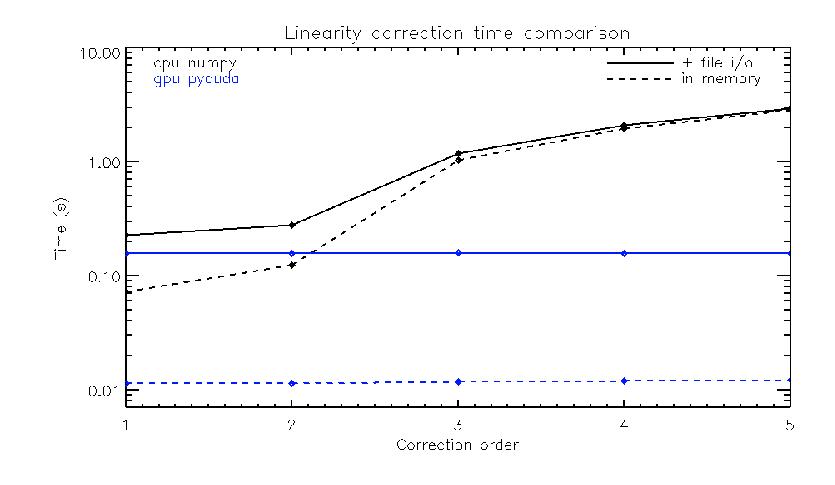
\includegraphics{part4/Warner_O31/O31_f1.eps}
\caption{File I/O is negligible compared to computation time on CPU for 3$^{rd}$ order and higher linearity corrections but dominates GPU computation time!}
\end{figure}

We present a new, flexible data pipeline model that combines GPU-optimized  
algorithms with a new design that not only minimizes file I/O and
byte-swapping operations, but also copying of data to and from the GPU. 

\section{Methods \& Algorithms}

Our data pipeline model is built in a python framework.  We choose python
because it is an open-source, object-oriented language that has gained
significant momentum within the astronomical community in recent years.
There are a myriad of math and astronomy libraries that are freely available
for python and supported by a large and active development community.  In
addition, there are python modules that support XML parsing and connecting
to relational database management systems (RDBMS) such as mysql and
PostgreSQL.  The PyCUDA
(\url{http://mathema.tician.de/software/pycuda}) module and python's native
C-API allow us to easily integrate GPU-optimized CUDA code into our data
pipeline, and finally, using python allows us to re-use some algorithms
and classes, with only minor modifications, from previous data pipelines,
specifically the Florida Analysis Tool Born Of Yearning for high quailty
scientific data (FATBOY).  We use a machine with an Nvidia 580 GTX GPU for
all of our tests.

Our first challenge is to determine the best way to flexibly select and
describe the data to be processed and the processes and options to be
applied to the data.  Extensible Markup Language (XML) is ideally suited for
this task.  Using a simple XML configuration file, the user will be able to
describe their data, where it comes from, and what processes should be applied
to the data.  The data can be retrieved either from an instrument's data
handling system (DHS), from a local filesystem, or from an RDBMS.
 
In order to process data in near real-time at the telescope and provide
rapid feedback via a quick-look mechanism, we select a data pipeline design
that operates on a per-image basis instead of a per-process basis.  At the
telescope, we will have one image coming in from the instrument's DHS, 
and will want to apply previously created master calibration frames to this
image immediately and send the resulting science data to the quick-look tool.
Through this design and the use of recursive logic (Fig. 2), we can minimize
file I/O to one read and one write per image.  All processes will be
applied to the data in memory, with as many as possible combined into
single steps on the GPU to minimize both file I/O and memory copying
(e.g., linearity correction, dark subtraction, flat division, and applying
a bad pixel mask are all done in one method on the GPU and then the resulting
data is then copied back to host memory).  Master calibration frames are
created once and then stored in memory and reused.

\begin{figure}[!ht]
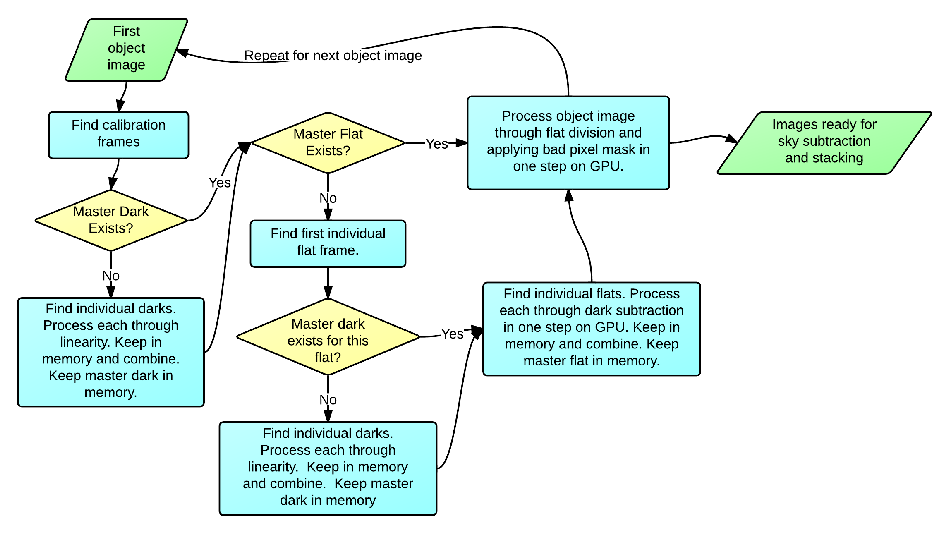
\includegraphics{part4/Warner_O31/O31_f2.eps}

\caption{Flow chart of recursive logic.  Master calibration frames are created
once when they are first requested and then stored in memory and reused.
All processes are applied to each frame in memory, with as many as possible
performed at once on the GPU, minimizing both file I/O and memory copying to and
from the GPU. }

\end{figure}


Finally, it is important that the data pipeline design be customizeable and
extensible so that new methods of both retrieving and processing data can be
easily added to suit the needs of particular instruments.  Our design provides
for this through the XML configuration file combined with the ability to
extend base classes and override methods as needed. 

\section{Results \& Conclusions}

Our preliminary results indicate that we can process a raw 2048 x 2048
near-infrared image all the way through sky subtraction and on-the-fly cosmic
ray removal and save the result
to disk in only 0.5 seconds!  This assumes that the master calibration frames
(dark, flat field, bad pixel mask, and sky) for this image are already stored
in memory.  The time required to create a master calibration frame depends
upon the number of images that compose it, but should generally be on the
order of 0.5 to 3 seconds.  With the exception of on-source skies, these
calibration frames will only be created once per dataset and then kept in
memory, minimizing overhead.

On-source skies are created from other object images at different positions
in the dither pattern and increase in quality with more frames.  However,
since the time required to create master sky frame is generally going to be
shorter than the exposure time for each observation, it will even be
possible to recreate an iteratively better master sky and redo the sky
subtraction after each observation in the dither pattern.  These iteratively
better sky subtracted images can then be updated on disk and in the
quick look tool, concurrent with continuing observations.  This will
considerably optimize the observing process, resulting in huge savings of
resources, money, and precious observing time.  We also believe that when
applied to large archives of data, this design will make it possible to
achieve a speed gain of as much as a factor of 30-40 over traditional
CPU-based data pipelines. 
